\documentclass[a4paper]{report}
\usepackage{tikz}
\usepackage[utf8]{inputenc}
\usepackage{amssymb}
\usepackage{amsmath}

\usetikzlibrary{arrows}

\title{Architecture\\GRT}

\begin{document}
\maketitle
\chapter{DPO graph rewriting approach}
Given a rule $L \overset{l}{\leftarrowtail} K \overset{r}{\rightarrowtail} R$ and a graph $G$, the DPO approach to graph rewriting is to commute the following diagram

\begin{center}
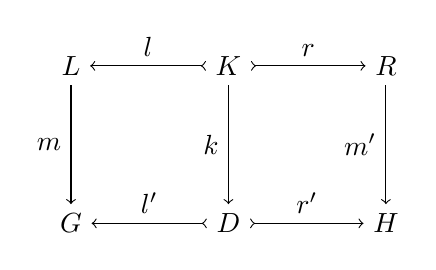
\begin{tikzpicture}
	\node (L) at (0,2) {$L$};
	\node (K) at (2,2) {$K$};
	\node (R) at (4,2) {$R$};
	\node (G) at (0,0) {$G$};
	\node (D) at (2,0) {$D$};
	\node (H) at (4,0) {$H$};

	\path[>->] (K) edge node [above] {$l$} (L);
	\path[>->] (K) edge node [above] {$r$} (R);
	\path[>->] (D) edge node [above] {$l'$} (G);
	\path[>->] (D) edge node [above] {$r'$} (H);
	\path[->] (R) edge node [left] {$m'$} (H);
	\path[->] (L) edge node [left] {$m$} (G);
	\path[->] (K) edge node [left] {$k$} (D);
\end{tikzpicture}
\end{center}
in which both squares are pushouts.

The morphisms in this diagram are:
\begin{itemize}
	\item $m$: is a homomorphism detection algorithm. In the diagram, $m$ is a single homomorphism, non-deterministically detected, but ideally, the algorithm should return all possible homomorphisms from $L$ to $G$. It is calculated.

	A second view of such morphism is that it is the set of arrows that maps $a \mapsto b, a \in L, b \in G$.

	\item $l, l', r, r'$ are all inclusions (supose that each one of them can be generically identified by $\phi : S \to T$). $\phi$ can be defined as the identities of the elements of the graph $T \backslash S$, and the inverse morphism $\phi^{-1}: T \nrightarrow S$ is a partial morphism that excludes nodes and edges in $T \backslash S$.

	\item $k, m'$: are morphisms derived from $m$. $k$ has the arrows of $m$ which the source is removed by $l^{-1}$ removed, along with the target of such arrows. $m'$ adds arrows to $k$, with source in the elements of $R \backslash K$ and target in the elements of $H \backslash D$.
\end{itemize}

These are all structure preserving. Two conditions impede the transformation to be applied:
\begin{itemize}
	\item \textit{dangling condition}: If after the deletion of a node, an edge is left ``dangling'', i.e. the node deleted was the source or target of an edge that was not removed.
	\item \textit{identification condition}: if an element is both deleted and maintained.
\end{itemize}

\chapter{Representation and algorithms}
\section{Graph}
A graph is represented by two sets $V$ of vertices and $E$ of edges. Each element must have an numerical identity. Edges must contain also a pair of node identites that are the source and target of an edge.

\section{Morphisms}
A morphism between graphs is represented by two lists of pairs: node and edge identities. The first element is the source of the morphism and the second element is the target of the morphism. one of them can be $\bot$ (\texttt{Nothing}), meaning that the element is created (when in the source) or deleted (when in the target). For the DPO approach, the source of each pair must be unique, except for $\bot$. 

\subsection{Decomposing morphisms}
\label{ssec:actions}
Morphisms can be decomposed in simple actions of adding, removing and keeping nodes and edges. These actions are encoded in the pairs of a morphism, as such:

\begin{tabular}{lll}
\textbf{Pair} & \textbf{Action on nodes} & \textbf{Action on edges} \\
$(s, s)$ & \texttt{keepNode n g} & \texttt{keepEdge e g} \\
$(s, \bot)$ & \texttt{delNode n g} & \texttt{delEdge e g} \\
$(\bot, s)$ & \texttt{addNode n g} & \texttt{addEdge e g} \\
$(s, t)$ & reserved for future use & reserved for future use \\
$(\bot, \bot)$ & \texttt{id g} & \texttt{id g} \\
\end{tabular}

\subsection{Application Order}
\label{ssec:order}
The operations must be applied in the following order to conform to the DPO approach:
\begin{enumerate}
	\item \texttt{removeEdge}
	\item \texttt{removeNode}
	\item \texttt{addNode}
	\item \texttt{addEdge}
	\item \texttt{keepNode}, \texttt{keepEdge}
\end{enumerate}

This, and the error condition and corrections below, gurantee the two application conditions of the DPO approach. The reasoning behind the claim is discussed after presenting the error conditions and corrections.

\subsection{Errors in morphism application}
Error conditions and correction (whenever possible) for such morphisms are:
\begin{itemize}
	\item when keeping an element, the element kept must exist; if it doesn't, an error must be returned. 
	\item In \texttt{addNode}, the node must not have the same identity of an existing node, but the identity can be remapped to a new name. This remapping will be discussed in the future.
	\item In \texttt{addEdge}, the two nodes it points to must exist in the graph; if not, it must return an error.
	\item In \texttt{removeEdge}, the edge must exist. Otherwise, an error must be returned.
	\item In \texttt{removeNode}, the node removed must not be pointed by any edge in the graph. If so, the actions must return an error.
\end{itemize}

\subsection{Inverting morphisms}
Inverted morphisms in Graph are morphism in which source and target are flipped. To invert a morphism, the action must flip each pair of edges and nodes in a given morphism.

\subsection{Remapping identities}
An operation of remapping the identities (names) of the elements of a graph is useful. A generic remap must receive a morphism, and a list of pairs (of nodes and edges) that indicate the way in which the remapping occurs; the first element is the original name, and the second is the new name.

When remapping a node identity, one must be careful to remap it's identity also in the edges. Edge name remapping can be by simply changing it's name. In both cases, the target must not exist in the graph prior to the remapping.

\subsection{DPO paradigm encoded in the actions}
One way to encode the DPO approach, using the actions described above, is to apply the following algorithm.

\begin{enumerate}
	\item Remap the target identities of the creation pairs $(\bot, t)$ to a set of identites that doesn't exist in the graph.
	\item Order the pairs as described in the Subsection \ref{ssec:order}.
	\item Convert each pair to the appropriate action, as described in Subsection \ref{ssec:actions}.
	\item \texttt{fold} the actions over the graph.
\end{enumerate}

In the end, either a graph or an error is returned. The error may or may not tell at which step the transformation failed.

\subsection{Action signatures}
\begin{verbatim}
keepEdge   :: (Monad m) => Edge b -> Digraph a b -> m (Digraph a b)
keepNode   :: (Monad m) => Node a -> Digraph a b -> m (Digraph a b)
addNode    :: (Monad m) => Node a -> Digraph a b -> m (Digraph a b)
addEdge    :: (Monad m) => Edge b -> Digraph a b -> m (Digraph a b)
removeEdge :: (Monad m) => Edge b -> Digraph a b -> m (Digraph a b)
removeNode :: (Monad m) => Node a -> Digraph a b -> m (Digraph a b)
\end{verbatim}

The reasoning for using a generic monad instead of \texttt{Maybe} is to allow for future modifications without having to modify the code completely. Actually, using only \texttt{return} to indicate a successful transformation, and \texttt{fail} with a descriptive message is sufficient for the actions described above.

\subsection{Morphism composition}


\section{Rules}
This morphism allows to describe a span $L \overset{l}{\leftarrowtail} K \overset{r}{\rightarrowtail} R$ as follows.

\begin{itemize}
	\item $L$ are all sources $s$ that are mapped to $\bot$ ($s \mid s \mapsto \bot$), plus all that are maintained ($s \mid s \mapsto s$).
	\item $R$ are all targets $t$ that are mapped from $\bot$ ($t \mid \bot \mapsto t$), plus all that are maintained ($t \mid t \mapsto t$).
	\item $K$ are all item that are maintained ($k \mid k \mapsto k$).
	\item $l$ are all pairs that the target is $\bot$ ($(s, \bot) \mid s \mapsto \bot$).
	\item $r$ are all pairs which the source if $\bot$ ($(\bot, t) \mid \bot \mapsto t$).
\end{itemize}

\section{Builders}
Builders are monadic interfaces to building graphs and rules in a simpler way. Both are based in the \texttt{StateT} monad to provide the basic functionality. They are planned to be composable, inspired by parsec. The builders type signatures are

\begin{verbatim}
type GraphBuilder a b m c = StateT (TypedDigraph a b) m c
type RuleBuilder a b m c = StateT (TypedDigraph a b, Rule a b) m c
\end{verbatim}

\subsection{Graph builder}
The graph builder provides the following functions:
\begin{verbatim}
-- Element creation
typeNode  :: Monad m => a -> GraphBuilder a b m Int
typeEdge  :: Monad m => b -> (Int, Int) -> GraphBuilder a b m Int
graphNode :: Monad m => a -> GraphBuilder a b m Int
graphEdge :: Monad m => b -> (Int, Int) -> GraphBuilder a b m Int

-- Element deletion
deleteTypeNode  :: Monad m => Int -> GraphBuilder a b m ()
deleteTypeEdge  :: Monad m => Int -> GraphBuilder a b m ()
deleteGraphNode :: Monad m => Int -> GraphBuilder a b m ()
deleteGraphEdge :: Monad m => Int -> GraphBuilder a b m ()
\end{verbatim}

A sample usage can be seen below.

\begin{verbatim}
tGraph :: Monad m => GraphBuilder m (Int, Int, Int, Int, Int, Int)
tGraph = do n1 <- typeNode
            n2 <- typeNode
            e1 <- typeEdge (n1, n1)
            e2 <- typeEdge (n2, n2)
            e3 <- typeEdge (n1, n2)
            e4 <- typeEdge (n2, n1)
            return (n1, n2, e1, e2, e3, e4)

beta :: Monad m => m (TypedDigraph () ())
beta = buildGraph $ do (tn1, tn2, te1, te2, te3, te4) <- tGraph
                       n1 <- graphNode tn1
                       n2 <- graphNode tn2
                       n3 <- graphNode tn1
                       n4 <- graphNode tn2
                       e1 <- graphEdge te1 (n1, n3)
                       return ()
\end{verbatim}

\subsection{Rule builder}
Similar to the graph builder.

\subsection{Algebraic iterface}

\end{document}